\documentclass{article}
\usepackage{geometry}
\geometry{
 a4paper,
 total={170mm,257mm},
 left=20mm,
 top=20mm,
}

\usepackage[OT1]{fontenc}
\renewcommand*\familydefault{\sfdefault}

\usepackage{graphicx}
\usepackage[utf8]{inputenc}
\usepackage[english]{babel}
\usepackage[english]{isodate}
\usepackage[parfill]{parskip}
\usepackage[hybrid]{markdown}

\usepackage{colortbl}
\usepackage{array}
\usepackage{booktabs}

\usepackage{xcolor}
\definecolor{ampliproblue}{RGB}{0, 77, 255}
\usepackage{sectsty}
\sectionfont{\color{ampliproblue}}
\subsectionfont{\color{ampliproblue}}
\subsubsectionfont{\color{ampliproblue}}

\markdownSetup{
  pipeTables,
  tableCaptions,
  rendererPrototypes = {
    image = {\begin{center}\setkeys{Gin}{width=.99\linewidth}\includegraphics{#2}\end{center}}, % center images inline expanding to page width
    codeSpan = {\texttt{#1}}, % Render inline code via `\texttt`.'
  }
}
\title{
  \textbf{\raisebox{-0.475em}{
\includegraphics[height=1.65em]{imgs/amplipro_nobg.png}} Expansion Unit - User Manual}
}
\date{}
\setlength\parindent{0pt}
\begin{document}

\maketitle
\setkeys{Gin}{width=.99\linewidth}
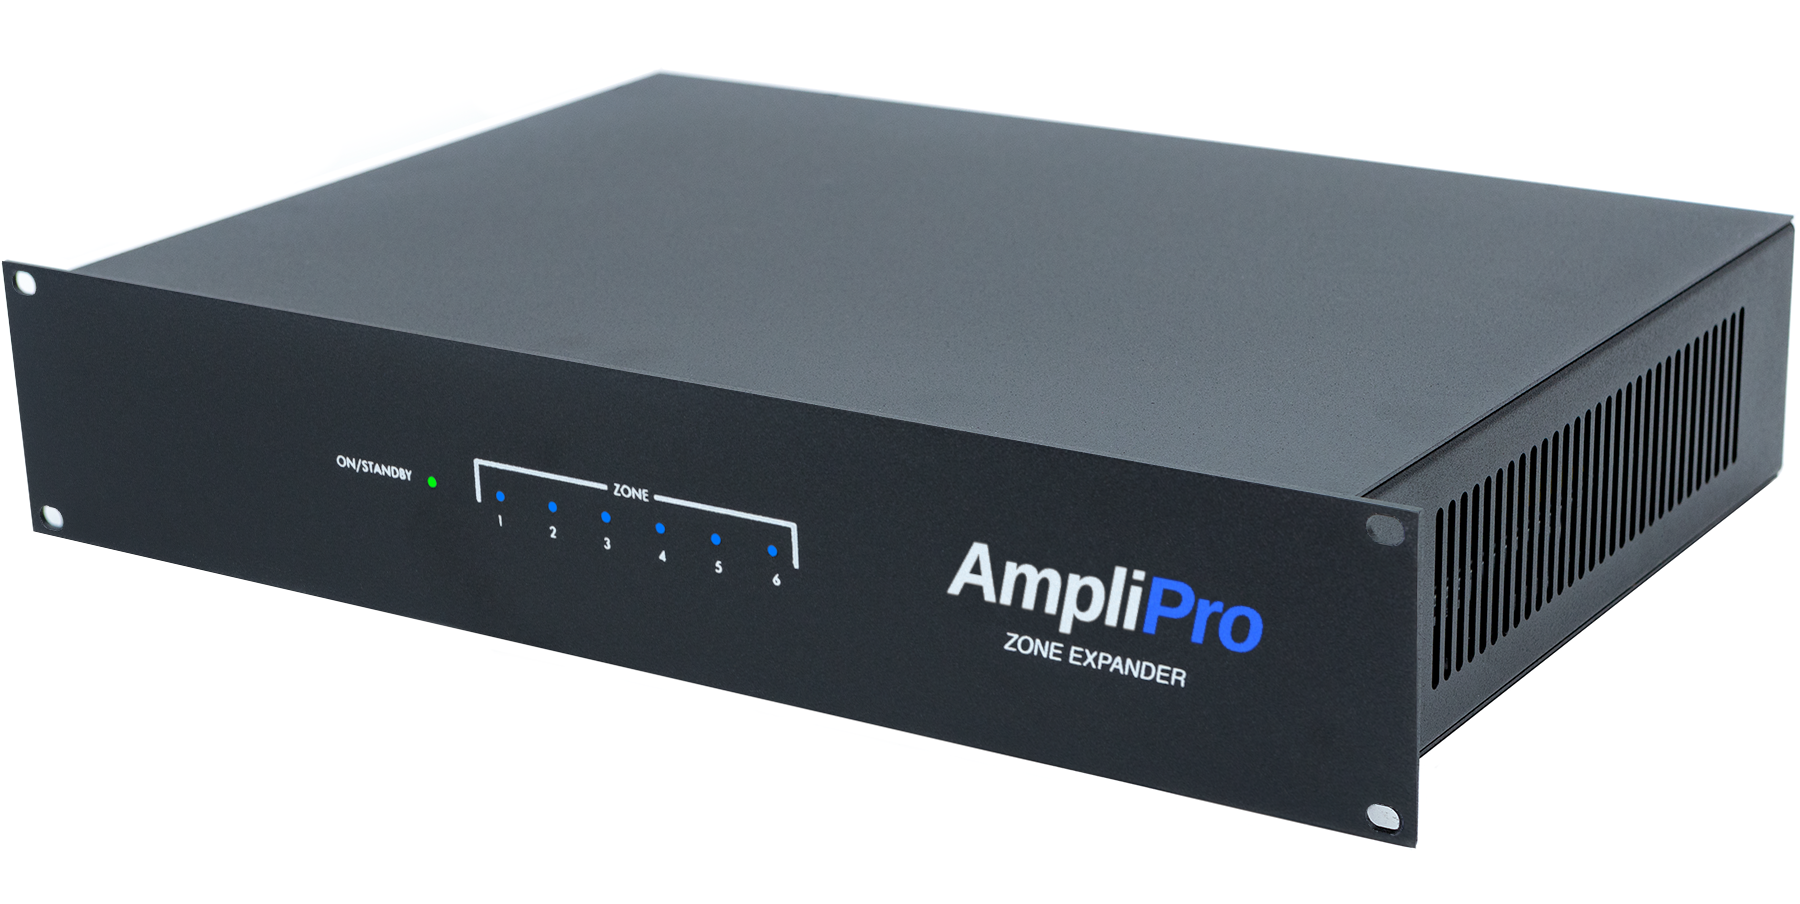
\includegraphics{ expander/sideview_expansion.png}
\begin{center}
  \LARGE{ \textbf{ Device Model: AP1-Z6}}
\end{center}

\includegraphics{ imgs/MicroNova_Logo.jpg}

\thispagestyle{empty}
\newpage
\thispagestyle{empty}
\tableofcontents
\newpage
\pagenumbering{arabic}

\markdownInput{common/LINKS.md}
\newpage
\markdownInput{common/SAFETY.md}
\newpage
\markdownInput{common/FCC.md}
\newpage
\markdownInput{expander/OVERVIEW.md}
\newpage
\markdownInput{common/SPECS_TITLE.md}
\renewcommand{\arraystretch}{2}
\rowcolors{2}{gray!25}{white}
\setlength{\arrayrulewidth}{0.5mm}

\resizebox{\textwidth}{!}{
  \begin{tabular}{|p{4cm}|p{10cm}|}
  \hline
  \textbf{Feature} & \textbf{Description} \\
  \hline

  Dimensions
  &
  2U 19" rackmount unit with 300mm depth, 12.5” L x 19” W x 3.5” H \\

  \hline

  Weight
  &
  15 lbs / 6.8 kg \\

  \hline

  Power Input
  &
  100-240VAC 50-60Hz max input 45W \\

  \hline

  Power Consumption
  &
  6.7W Idle \newline
  391W Continuous \newline
  782W Peak \\

  \hline

  Peak Current Consumption
  &
  6.8A @ 115VAC or 3.4A @230VAC \\

  \hline

  Outputs
  &
  4 x Line-Level RCA \newline Ch 1: up to 32-bit 384 kHz DAC output \newline Ch 2-4: up to 16-bit 48 kHz DAC output \\

  \hline

  Speaker Power
  &
  55 WPC @ 4 Ω \newline
  32 WPC @ 8 Ω \\

  \hline

  Speaker Power
  &
  55 WPC @ 4 Ω \newline
  32 WPC @ 8 Ω \\

  \hline

  Speaker Impedance
  &
  4 - 8 Ω \\

  \hline

  Speaker Zones
  &
  6, Expandable up to 36 with AmpliPro Expansion Units\\

  \hline

  Inputs
  &
  1 x Chain In (audio from Chain Out from main unit) \\

  \hline

  Digital Audio Sources
  &
  32-bit 384KHz (Source 1), 16-bit 48KHz (Sources 2, 3, 4) \\

  \hline
  \end{tabular}
}

\newpage
\markdownInput{expander/INSTALLATION.md}
\newpage
\markdownInput{common/TROUBLESHOOTING.md}
\newpage
\markdownInput{common/WARRANTY.md}
\newpage
\markdownInput{common/GLOSSARY.md}

\end{document}
